\chapter{Introduction to Hamiltonian Systems}
A canonical Hamiltonian system is given by two state variables $p,q \in \mathbb{R}^{n}$ (i.e. the entire system is even dimensional), a \emph{Hamiltonian} function $H(p,q,t)\in \mathcal{C}^{1}(\mathbb{R}^{2n}\times \mathbb{\mathbb{R}})$ which maps $\mathbb{R}^{n}\times\mathbb{R}^{n}\times\mathbb{R}\to \mathbb{R}$. In general $q$ denotes the generalized coordinates (position) and $p$ the generalized velocities (momentum). The dynamics on the system are given by
\begin{align}
	\begin{dcases}
		\dot{q} = \frac{\partial H(q,p,t)}{\partial p}\\
		\dot{p} = - \frac{\partial H(q,p,t)}{\partial q}.
	\end{dcases}
\end{align}
This is represented in shorthand notation by using the identity matrix, denoted by $I_{n}\in\mathbb{R}^{n\times n}$ and the symplectic matrix
\begin{align}
	J = 
	\begin{pmatrix}
		0 & I_{n}\\
		-I_{n} & 0
	\end{pmatrix}
.	
\end{align}
Denote the differential with respect to the state variables $x =
\begin{pmatrix}
	p \\ q
\end{pmatrix}
\in \mathbb{R}^{2n}$ by
\begin{align}
	D_{x} = D = 
	\begin{pmatrix}
		\frac{\partial}{\partial q} \\
		\frac{\partial}{\partial p}
	\end{pmatrix}
.	
\end{align}
Then the shorthand notation for the system is
\begin{align}
	\boxed{
	\dot{x} = JD_{x}H(x,t).
}
\end{align}

\begin{ex}[Holonommic mechanical systems are Hamiltonian]
	Assume that all external forces are derived from a potential, i.e. $F(q,t)= -\frac{\partial V(q,t)}{\partial q}$ where $q$ denotes the position. Further assume that all constraints are geometric, i.e. $f(q,t)=0$. We have $n$ degrees of freedom as $q \in \mathbb{R}^{n}$ and $\dot{q} \in \mathbb{R}^{n}$. The kinetic energy is given by $T(q,\dot{q})$ and the potential energy by $V(q,t)$. We then use Newton's second law which is equivalent to the principle of least action (Maupertius's principle). This principle states that for the \emph{Lagrangian} $L = T-V$ we have that the variational derivative of the action is 0
	\begin{align}
		\boxed{
			\delta \int_{t_0}^{t_1} L(q(s), \dot{q}(s), s)ds = 0. \numberthis \label{eq8:ELE} 
	}
	\end{align}
	This implies the \emph{Euler-Lagrange equations}
	\begin{align}
\frac{d}{dt} \frac{\partial L}{\partial \dot{q}} - \frac{\partial L}{\partial q} = 0.	
	\end{align}
Thus we have $n$, second-order ODEs. 

\begin{remark}[]
	In \eqref{eq8:ELE} the variational derivative $\delta$ being equal to 0 stems from the principle of least action, as the action $\int_{}^{} L(q(s), \dot{q}(s), s)ds$ is then a minimum. The variational derivative $\delta$ of a functional $F$ (here $F[\gamma]=\int_{}^{} \gamma ds)$ of a path (in our case $\gamma = (q(s), \dot{q}(s), s)$) corresponds to seeing how infinitesimal changes to the path change the output of the functional. These different paths are depicted in Fig. \ref{fig:variational_deriv}.
	\begin{figure}[h!]
		\centering
		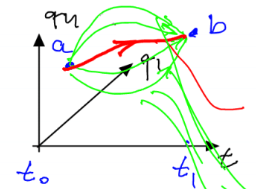
\includegraphics[width=0.35\textwidth]{figures/ch8/1variational_deriv.png}
		\caption{An illustration of various different paths (denoted here by $q(t)$). The red demarcates the actual motion which occurs in the system, whereas the green paths are each admissible motions which are consistent with the constraints.}
		\label{fig:variational_deriv}
	\end{figure}
\end{remark}
Now assume that $L$ is a convex function of $\dot{q}$. Using this the \emph{Legendre transfomation} of $L$ can be performed, which is essentially just a different way to look at the graph of $L(q, \cdot, t)$. This transformation gives us
\begin{align}
	H\left(q, \frac{\partial L}{\partial \dot{q}}, t\right) = \frac{\partial L}{\partial \dot{q}}\dot{q} - L(q, \dot{q}, t).
\end{align}
Th geometric interpretation of this is shown in Fig. \ref{fig:legendre_trafo}. At each velocity $\dot{q}$ the tangent line of $L(q, \cdot, t)$ is taken and shifted such that the $y$-intercept is at $0$. Then $H$ is equal to the difference between this shifted line and the function $L(q, \dot{q}, t)$.
\begin{figure}[h!]
	\centering
	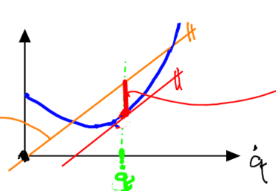
\includegraphics[width=0.35\textwidth]{figures/ch8/2legendre_trafo.png}
	\caption{The Legendre transformation. The thin red linear function denotes the tangent of $L(q, \cdot, t)$ taken at  $\dot{q}$, the yellow linear function is then the shifted version with a 0 $y$-intercept, and the thick red vertical line is the Legendre transformation $H$ measuring the difference between this shifted line and $L(q,\cdot, t)$.}
	\label{fig:legendre_trafo}
\end{figure}

As $L$ is convex, if we define the generalized momenta $p=\frac{\partial L}{\partial \dot{q}}$. There then exists a unique $\dot{q}$ such that $\dot{q} = F(q,p,t)$, in fact the relationship between $\dot{q}$ and $p$ here is 1:1 (bijective). We then have
\begin{align}
	H(q,p,t) = p F(q,p,t) - L (q, F(q,p,t), t)
\end{align}
the Hamiltonian associated with $L$ (or the Legendre transform of $L$).

At this point note that
\begin{align}
	dH &= \frac{\partial H}{\partial q}dq + \frac{\partial H}{\partial p}dp + \frac{\partial H}{\partial t}dt \\
	   &= d(pF) - \underbrace{\frac{\partial L}{\partial q}}_{=\dot{p}} dq - \underbrace{\frac{\partial L}{\partial \dot{q}}}_{=p} - \frac{\partial L}{\partial t}dt \\
	   &= \underbrace{F}_{=\dot{q}}dp + pdF - \dot{p}dq - pdF - \frac{\partial L}{\partial t}dt \\
	   &= \dot{q}dp - \dot{p}dq - \frac{\partial L}{\partial t}dt.
\end{align}
Comparing coefficients in the first and last equations then yields
\begin{align}
	\begin{dcases}
		\dot{q} = \frac{\partial H}{\partial p}\\
		\dot{p} = -\frac{\partial H}{\partial q}
	\end{dcases}
.	
\end{align}
This first-order ODE is called the \emph{Hamiltonian equations of motion}. The meaning of the Hamiltonian is $H= 2T - (T-V) = T+V = T(q,p,t) + V(q,t)$, the full mechanical energy. Also note that we have $\frac{\partial H}{\partial t} = - \frac{\partial L}{\partial t}$.
\end{ex}

We will now apply this result to a well known system.

\begin{ex}[The Hamiltonian of the pendulum]
	Recall that for the pendulum the position is given by $q=\varphi\in S^{1}$, with a string of length $\ell$ the vertical deflection of the pendulum is $\ell(1- \cos(\varphi)$. The string is assumed massless and the mass at the end of the string is given by $m$. 
	
	We have the kinetic and potential energy 
	\begin{align}
		T = T(\dot{q}) = \frac{1}{2} m (\ell \dot{\varphi})^{2} = \frac{1}{2} m\ell^2 \dot{\varphi}^{2};\quad V = V(q) = mg\ell(1-\cos(\varphi)).
	\end{align}
Therefore the Lagrangian is given by
\begin{align}
	L = T-V = \frac{1}{2}m \ell^2 \dot{\varphi}^{2} - mg\ell(1-\cos(\varphi)).
\end{align}
To find the generalized momentum, we calculate the partial derivative of the Lagrangian with respect to $\dot{q}$, i.e.
\begin{align}
p = \frac{\partial L}{\partial \dot{q}} = \frac{\partial L}{\partial \dot{\varphi}} = m\ell^2 \dot{\varphi}\implies \dot{\varphi} = \frac{p}{m\ell^2}.
\end{align}
Now it is possible to calculate the Hamiltonian
\begin{align}
	H = p \frac{p}{m\ell^2} - \frac{1}{2}m\ell^2 \frac{p^2}{(m\ell^2)^2} + mg\ell(1-\cos(\varphi))
	= \underbrace{\frac{1}{2} \frac{p^2}{m\ell^2}}_{T} + \underbrace{mg\ell(1-\cos(\varphi))}_{V}.
\end{align}
Hence for this Hamiltonian system we have the Hamiltonian equations of motion
\begin{align}
\begin{dcases}
	\dot{\varphi} = \frac{\partial H}{\partial p} = \frac{p}{m\ell^2} \\
	\dot{p} = - \frac{\partial H}{\partial q} = -mg\ell \sin (\varphi).
\end{dcases}
\end{align}
\end{ex}

\begin{ex}[2-dimensional incompressible fluids are Hamiltonian]
	We begin on a domain $\mathcal{D}$ contained on the plane which is simply connected, i.e. it has no holes. For each position $x\in \mathcal{D}$ we have the velocity field
	\begin{align}
		{V}(x,t) = 
		\begin{pmatrix}
			u(x,y,t) \\ v(x,y,t)
		\end{pmatrix},
	\end{align}
	i.e. for each position we have
	 \begin{align}
		\begin{pmatrix}
			\dot{x} \\ \dot{y}
		\end{pmatrix}
		= 
		\begin{pmatrix}
			u \\v
		\end{pmatrix}
		.
	\end{align}
The incompressibility condition is given by 
\begin{align}
	\nabla \cdot V = \frac{\partial u}{\partial x} + \frac{\partial v}{\partial y}= 0\quad \forall x\in \mathcal{D}\subset \mathbb{R}^{2}.
\end{align}
Now rewrite this as a 3-dimensional equation
\begin{align}
	\nabla \times 
	\begin{pmatrix}
		-v \\ u \\ 0 
	\end{pmatrix}
	=0 \Leftrightarrow
	\nabla \cdot V = 0.
\end{align}
The third component here $\frac{\partial u}{\partial x} =  \frac{\partial -v}{\partial y}= \frac{\partial u}{\partial x} - \frac{\partial v}{\partial y}=0$. On $\mathcal{D}\times \mathbb{R}$ (which is simply connected in $\mathbb{R}^{3}$) the vector field $
\begin{pmatrix}
	-v \\ u \\ 0
\end{pmatrix}
$ has zero curl. Therefore there exists a potential of this vector field $\Psi:\mathcal{D}\times \mathbb{R} \to \mathbb{R}$ such that
\begin{align}
\begin{pmatrix}
	-v \\ u \\ 0 
\end{pmatrix}
 = \nabla \Psi =
 \begin{pmatrix}
 	\partial_x \Psi \\ \partial_y \Psi \\ \partial_z \Psi
 \end{pmatrix}
 \implies \Psi = \Psi(x,y,t).
\end{align}
Therefore we find
\begin{align}
	\begin{dcases}
		-\dot{y} = \frac{\partial \Psi}{\partial x} \\
		\dot{x} = \frac{\partial \Psi}{\partial y}
	\end{dcases}
	\implies 
	\begin{dcases}
		\dot{x} = \frac{\partial \Psi(x,y,t)}{\partial y} \\
	\dot{y} = -\frac{\partial \Psi(x,y,t)}{\partial x}.
	\end{dcases}
\end{align}
Thus we have shown that particle motion is Hamiltonian.
\end{ex}

\begin{ex}[Planar, Autonomous dynamical systems with a conserved quantity are Hamiltonian]
	We begin with the dynamical system which has a first integral $U$ (which is not constant), i.e.
	\begin{align}
		\dot{x} = f(x);\quad x \in \mathbb{R}^{2};\quad \exists U:\mathbb{R}^{2}\to \mathbb{R}:\ \frac{dU(x(t))}{dt}=0.
	\end{align}
	Note that this first integral property has further implications
	\begin{align}
		\frac{dU(x(t))}{dt} = DU(x(t)) \cdot \dot{x}(t) = DU \cdot \left.f\right|_{x(t)} = 0 \implies DU \perp f.
	\end{align}
Therefore, we can take the orthogonal complement of $DU$ and scale this to be equal to $f$, i.e.
\begin{align}
	f(x) = p(x) JDU(x) \implies \dot{x} = p(x) JDU(x).
\end{align}
Such a system is called a \emph{generalized Hamiltonian system} with the scalar function $p(x)$. Here the symplectic matrix in 2 dimensions is given by the $90^{\degree}$ rotation
\begin{align}
	J = 
	\begin{pmatrix}
		0 & I_{1}\\
		-I_{1} & 0 
	\end{pmatrix}
	=
	\begin{pmatrix}
		0 & 1 \\
		-1 & 0
	\end{pmatrix}
	.
\end{align}
If we assume $p(x)\neq0$ for all $x\in \mathcal{D} \subset \mathbb{R}^{2}$ then we may defined the trajectory-dependent rescaling of time
\begin{align}
	\tau = \int_{0}^{t} p(x(s))ds.
\end{align}
Then, define the notation for the derivative with respect to $\tau$ as follows
 \begin{align}
	 \frac{d(\ )}{dt} = \frac{d(\ )}{d\tau} \underbrace{\frac{d\tau }{dt}}_{p(x(t))} = (\ )' p.
\end{align}
Hence, using this time-transformation we have
\begin{align}
	\dot{x} = pJDU \implies x'p = pJDU \implies \boxed{x' = JDU(x).}
\end{align}
Therefore, we have a canonical Hamiltonian system. In fact, all planar, autonomous systems with a nontrivial first integral are Hamiltonian systems after a possible reparameterization of time.
\end{ex}

\begin{remark}[]
	The fact that the first integral was not trivial (i.e. non-constant) is critical, as otherwise $DU$ would be constantly 0, as we must be able to phrase the right hand side $f$ in terms of $DU$. Only in the case $f=0$ would this then be possible.
\end{remark}

\begin{ex}[Lotka-Volterra model (1925) for predator-prey interactions]
	For more information about this model see \cite{Lotka1925, Volterra1926}. Let the size of the prey population be represented by $h(t)$ and the size of the predator population be denoted by $p(t)$. Each of these populations must be at least 0. Now for strictly positive constants $a_1$, $a_2$, $b$, and $c$ we have the following dynamics
	\begin{align}
		\begin{dcases}
			\dot{h} = a_1 h(1- bp) \\
			\dot{p} = -a_2 p(1-ch).
		\end{dcases}
	\end{align}
	The phase portrait of this system is depicted in Fig. \ref{fig:lotka_volterra}.
	\begin{figure}[h!]
		\centering
		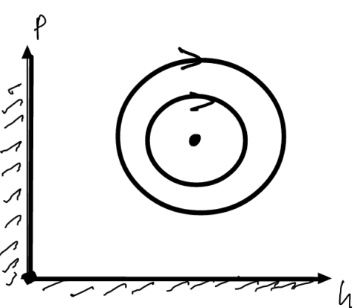
\includegraphics[width=0.3\textwidth]{figures/ch8/3lotka_volterra.png}
		\caption{The phase portrait of the Lotka-Volterra dynamics, such a dynamics has been used to explain the observed cycles in fish populations.}
		\label{fig:lotka_volterra}
	\end{figure}

	This system does in fact have a first integral, and thus it is Hamiltonian.	
\end{ex}

Now that we have seen multiple examples of Hamiltonian systems, we would like to better understand what properties they all share.

\section{Properties of Hamiltonian systems}
The setup going forward will be as follows for $n\geq 1$
\begin{align}
	\dot{x} = JDH(x,t);\quad x=
	\begin{pmatrix}
		q \\ p
	\end{pmatrix}
	\in \mathbb{R}^{2n};\quad 
	J=
	\begin{pmatrix}
		0 & I_n\\
		-I_n & 0 
	\end{pmatrix}.\numberthis \label{eq8:hamiltonian}	
\end{align}
\begin{proposition}[Conservation of the Hamiltonian (energy)]
	If $\frac{\partial H}{\partial t}=0$ (i.e. $H$ is only a function of $q$ and $p$) then $H(x(t))$ is constant on all trajectories. Therefore $H(x)$ is a first integral.	
\end{proposition}
\begin{proof}
	Use $J = -J^{T}$ to calculate
	\begin{align}
		\frac{dH(x(t))}{dt} = DH(x(t)) \cdot JDH(x(t)) = \left.\langle DH, JDH \rangle \right|_{x= x(t)} = 0.
	\end{align}
\end{proof}
The \emph{energy surface} for some constant $H_0$ $E_{0}=\left\{ x \in \mathbb{R}^{2n}:\ H(x)= H_0 \right\} $ is an invariant surface for the system. By nature of this $JDH$ must be tangent to $E_0$. Assuming that $E_0$ contains no fixed points of \eqref{eq8:hamiltonian} is equivalent to $DH(x_0)\neq 0$ for all $x_0$ in $E_0$. Hence, by the Implicit Function Theorem, the solution of $H(x)-H_0=0$ can be smoothly continued from $x_0$. Indeed, we have
\begin{align}
	DH(x_0)\neq 0\in \mathbb{R}^{2n} \implies \exists i:\ \left.\frac{\partial H}{\partial x^{i}}\right|_{x=x_0} \neq 0.
\end{align}
Then we have $x^{i}=F\left(x^{1},\ldots,x^{i-1},x^{i+1},\ldots,x^{2n}\right)$ for $F\in \mathcal{C}^{1}$, because $H$ is smooth. This implies that $E_{0}$ is a smooth $2n-1$-dimensional graph (i.e. a smooth hypersurface or codimension-one surface).
